\documentclass[]{article}
\usepackage[T1]{fontenc}
\usepackage{lmodern}
\usepackage{amssymb,amsmath}
\usepackage{ifxetex,ifluatex}
\usepackage{fixltx2e} % provides \textsubscript
% use upquote if available, for straight quotes in verbatim environments
\IfFileExists{upquote.sty}{\usepackage{upquote}}{}
\ifnum 0\ifxetex 1\fi\ifluatex 1\fi=0 % if pdftex
  \usepackage[utf8]{inputenc}
\else % if luatex or xelatex
  \ifxetex
    \usepackage{mathspec}
    \usepackage{xltxtra,xunicode}
  \else
    \usepackage{fontspec}
  \fi
  \defaultfontfeatures{Mapping=tex-text,Scale=MatchLowercase}
  \newcommand{\euro}{€}
\fi
% use microtype if available
\IfFileExists{microtype.sty}{\usepackage{microtype}}{}
\usepackage{longtable,booktabs}
\usepackage{graphicx}
% Redefine \includegraphics so that, unless explicit options are
% given, the image width will not exceed the width of the page.
% Images get their normal width if they fit onto the page, but
% are scaled down if they would overflow the margins.
\makeatletter
\def\ScaleIfNeeded{%
  \ifdim\Gin@nat@width>\linewidth
    \linewidth
  \else
    \Gin@nat@width
  \fi
}
\makeatother
\let\Oldincludegraphics\includegraphics
{%
 \catcode`\@=11\relax%
 \gdef\includegraphics{\@ifnextchar[{\Oldincludegraphics}{\Oldincludegraphics[width=\ScaleIfNeeded]}}%
}%
\ifxetex
  \usepackage[setpagesize=false, % page size defined by xetex
              unicode=false, % unicode breaks when used with xetex
              xetex]{hyperref}
\else
  \usepackage[unicode=true]{hyperref}
\fi
\hypersetup{breaklinks=true,
            bookmarks=true,
            pdfauthor={},
            pdftitle={},
            colorlinks=true,
            citecolor=blue,
            urlcolor=blue,
            linkcolor=magenta,
            pdfborder={0 0 0}}
\urlstyle{same}  % don't use monospace font for urls
\setlength{\parindent}{0pt}
\setlength{\parskip}{6pt plus 2pt minus 1pt}
\setlength{\emergencystretch}{3em}  % prevent overfull lines
\setcounter{secnumdepth}{0}
\usepackage{fancyhdr}
\pagestyle{fancy}
\lhead{C-Lyrics - A Word Cloud for Lyrics}
\rhead{\thepage}
\cfoot{Team 6}
\renewcommand{\headrulewidth}{0.4pt}
\renewcommand{\footrulewidth}{0.4pt}

\title{Clyrics - A Word Cloud for Lyrics}
\author{Justine Cocchi\\jcocchi@usc.edu \and Kelsey Fargas\\kfargas@usc.edu \and Mark Krant \\ mkrant@usc.edu\and Milad Gueramian\\gueramia@usc.edu \and Jeff Kang\\kangjr@usc.edu \and Séb Arnold\\arnolds@usc.edu}
\date{30 March 2015}

\title{%
	C-lyrics - A Word Cloud for Lyrics \\
	\large Testing Report}

\begin{document}

\clearpage\maketitle
\thispagestyle{empty}

\pagebreak

\tableofcontents
\setcounter{tocdepth}{3}
\thispagestyle{empty}

\pagebreak

\section{Executive Summary}\label{executive-summary}

C-lyrics is a public website that will generate a word cloud for any
given artist based on the most frequently used words that appear across
all of the artist's published songs. This product will interface with
the EchoNest API which will serve as the database from which we find and
analyze the songs. By clicking on a specific word in the word cloud the
user can see a list of all of the songs that word appears in and how
frequently it occurs in each song. Furthermore, the user can click on
any listed song title to see the complete lyrics for that song with the
original word that was selected from the word cloud highlighted every
time it appears.

C-lyrics is intended for use by the general public. There will be no
login required and there is no stored history of previous searches.
Because of this we will have very low memory requirements and can run
the product off of one server. The user can access C-lyrics using any
device running any OS, assuming it has an internet connection. After
typing in the artist name and selecting the submit button, the word
cloud will be generated and will be able to be shared via Facebook.

\pagebreak

\section{1 Introduction}\label{introduction}

\subsection{1.1 Purpose}\label{purpose}

This software testing document is meant to explain, detail, and report
on the white-box and black box tests that are run on the implemented
software code in order to assure quality. In addition, coverage metrics,
justifications and processes will be described. The document also
includes project management plans and schedules that were used to
accomplish the testing phase.

\subsection{1.2 Overview}\label{overview}

C-Lyrics is implemented using 2 languages, PHP and JavaScript. The
backend is implemented using PHP while the front end is built using Java
Script with the Angular JS framework. We used the PHPUnit framework for
white box testing the back end PHP functions. However, we also needed to
perform some whitebox testing on the AngularJS frontend implementation.
To test code implemented using AngularJS we used the Karma testing
platform which works conveniently well for the purpose. To perform our
blackbox end-to-end tests we used the Protractor framework.

The document is therefore organized into two main sections, Unit
testing, and Acceptance testing. Details about each testing scenario are
explained in subsections of these two main sections. The project
management documentation can be found in the appendices which comprise
the last section of this document. \#\# \textbf{1.3 References} {[}1{]}
IEEE. IEEE Std 830-1998 IEEE Recommended Practice for Software
Requirements Specifications. IEEE Computer Society, 1998.

{[}2{]} ``word cloud''.
\href{http://www.oxforddictionaries.com/us/definition/american_english/word-cloud}{Oxforddictionaries.com}
(January 31, 2015)

{[}3{]} EchoNest API
\href{http://developer.echonest.com/docs/v4/index.html\#overview}{documentation}
(January 29, 2015)

{[}4{]} A document to remind us the definitions of each UML symbol
\href{http://loufranco.com/wp-content/uploads/2012/11/cheatsheet.pdf}{UML
Cheatsheet} (February 17, 2015)

{[}5{]} Gliffy, a tool to create flowcharts and diagrams.
\href{https://www.gliffy.com}{Gliffy.com} (February 17, 2015)

{[}6{]} Wikipedia definition of black-box testing.
{[}http://en.wikipedia.org/wiki/Black-box\_testing{]} (February 17,
2015)

{[}7{]} Wikipedia definition of white-box testing.
{[}http://en.wikipedia.org/wiki/White-box\_testing{]} (February 17,
2015)

\subsection{1.4 Definitions And
Acronyms}\label{definitions-and-acronyms}

\begin{longtable}[c]{@{}ll@{}}
\toprule\addlinespace
\begin{minipage}[t]{0.47\columnwidth}\raggedright
Term
\end{minipage} & \begin{minipage}[t]{0.47\columnwidth}\raggedright
Definition
\end{minipage}
\\
\hline
\\\addlinespace
\begin{minipage}[t]{0.47\columnwidth}\raggedright
AJAX
\end{minipage} & \begin{minipage}[t]{0.47\columnwidth}\raggedright
Asynchronous JavaScript And XML. Technology allowing the transfer of
data from between the front- and back-end without reloading the web
page.
\end{minipage}
\\\addlinespace
\begin{minipage}[t]{0.47\columnwidth}\raggedright
API (EchoNest)
\end{minipage} & \begin{minipage}[t]{0.47\columnwidth}\raggedright
API will refer to the EchoNest API. EchoNest is a free API that allows
developers to retrieve lyrics and artist information in web pages and
other programs.
\end{minipage}
\\\addlinespace
\begin{minipage}[t]{0.47\columnwidth}\raggedright
Autocomplete
\end{minipage} & \begin{minipage}[t]{0.47\columnwidth}\raggedright
Autocomplete refers to the functionality addition to the Search Bar,
allowing users to enter minimal characters and choose artists that are
most similar to the string and display a picture of those artists next
to their name.
\end{minipage}
\\\addlinespace
\begin{minipage}[t]{0.47\columnwidth}\raggedright
Autocomplete Delay
\end{minipage} & \begin{minipage}[t]{0.47\columnwidth}\raggedright
A feature designed for the search bar when a user is typing. The delay
refers to the suspending action while the user is typing, making the
request to the server for autocomplete.
\end{minipage}
\\\addlinespace
\begin{minipage}[t]{0.47\columnwidth}\raggedright
Backend
\end{minipage} & \begin{minipage}[t]{0.47\columnwidth}\raggedright
References the PHP backend page
\end{minipage}
\\\addlinespace
\begin{minipage}[t]{0.47\columnwidth}\raggedright
Back to home button
\end{minipage} & \begin{minipage}[t]{0.47\columnwidth}\raggedright
A button redirecting the user to the homepage.
\end{minipage}
\\\addlinespace
\begin{minipage}[t]{0.47\columnwidth}\raggedright
Back to songs button
\end{minipage} & \begin{minipage}[t]{0.47\columnwidth}\raggedright
A button redirecting the user to the songs list page.
\end{minipage}
\\\addlinespace
\begin{minipage}[t]{0.47\columnwidth}\raggedright
Commonly Used Web Browser
\end{minipage} & \begin{minipage}[t]{0.47\columnwidth}\raggedright
Browsers such as Firefox, Safari, Chrome, Explorer, and Quora which come
on mobile phones, tablets and personal computers.
\end{minipage}
\\\addlinespace
\begin{minipage}[t]{0.47\columnwidth}\raggedright
Customer/Client
\end{minipage} & \begin{minipage}[t]{0.47\columnwidth}\raggedright
Dr. William G. Halfond and Sonal Mahajan
\end{minipage}
\\\addlinespace
\begin{minipage}[t]{0.47\columnwidth}\raggedright
GitHub
\end{minipage} & \begin{minipage}[t]{0.47\columnwidth}\raggedright
A web service that provides software version control tools.
www.github.com
\end{minipage}
\\\addlinespace
\begin{minipage}[t]{0.47\columnwidth}\raggedright
Stakeholders
\end{minipage} & \begin{minipage}[t]{0.47\columnwidth}\raggedright
The client and the development team
\end{minipage}
\\\addlinespace
\begin{minipage}[t]{0.47\columnwidth}\raggedright
LOC
\end{minipage} & \begin{minipage}[t]{0.47\columnwidth}\raggedright
acronym: for Lines of Code
\end{minipage}
\\\addlinespace
\begin{minipage}[t]{0.47\columnwidth}\raggedright
KSLOC
\end{minipage} & \begin{minipage}[t]{0.47\columnwidth}\raggedright
a metric that stands for: 1,000(K) Source Lines of Code
\end{minipage}
\\\addlinespace
\begin{minipage}[t]{0.47\columnwidth}\raggedright
Desktop Platform
\end{minipage} & \begin{minipage}[t]{0.47\columnwidth}\raggedright
A screen whose width exceeds 560px
\end{minipage}
\\\addlinespace
\begin{minipage}[t]{0.47\columnwidth}\raggedright
Development Team
\end{minipage} & \begin{minipage}[t]{0.47\columnwidth}\raggedright
All of the individuals whose names appear on the cover of this document.
These persons have collectively put this document together and will
collectively implement the software product described in subsequent
sections.
\end{minipage}
\\\addlinespace
\begin{minipage}[t]{0.47\columnwidth}\raggedright
Facebook
\end{minipage} & \begin{minipage}[t]{0.47\columnwidth}\raggedright
Online social network service where the generated word cloud image may
be shared amongst users.
\end{minipage}
\\\addlinespace
\begin{minipage}[t]{0.47\columnwidth}\raggedright
FR
\end{minipage} & \begin{minipage}[t]{0.47\columnwidth}\raggedright
Functional Requirement
\end{minipage}
\\\addlinespace
\begin{minipage}[t]{0.47\columnwidth}\raggedright
Google Doc
\end{minipage} & \begin{minipage}[t]{0.47\columnwidth}\raggedright
An online service provided by Google Inc. where an editable document~can
be accessed and change simultaneously by the members who have been given
access to the document. In the case of the development team, google doc
is the shared resource which contains the source of this SRS document.
\end{minipage}
\\\addlinespace
\begin{minipage}[t]{0.47\columnwidth}\raggedright
Home Page
\end{minipage} & \begin{minipage}[t]{0.47\columnwidth}\raggedright
The first page of the website visited by the user. It contains the Word
Cloud as well as the Search Bar.
\end{minipage}
\\\addlinespace
\begin{minipage}[t]{0.47\columnwidth}\raggedright
Lyrics Page
\end{minipage} & \begin{minipage}[t]{0.47\columnwidth}\raggedright
The third page of the website, it contains the lyrics for one song,
which is chosen by the user on the Songs Page. It will have two
Navigation Buttons that can take the user to either the Home Page or
back to the Songs Page.
\end{minipage}
\\\addlinespace
\begin{minipage}[t]{0.47\columnwidth}\raggedright
Mobile Platform
\end{minipage} & \begin{minipage}[t]{0.47\columnwidth}\raggedright
A screen whose width is less than or equal to 560px
\end{minipage}
\\\addlinespace
\begin{minipage}[t]{0.47\columnwidth}\raggedright
MVC
\end{minipage} & \begin{minipage}[t]{0.47\columnwidth}\raggedright
The Model-View-Controller Software Pattern
\end{minipage}
\\\addlinespace
\begin{minipage}[t]{0.47\columnwidth}\raggedright
Navigation Buttons
\end{minipage} & \begin{minipage}[t]{0.47\columnwidth}\raggedright
Refers to any button that takes the user to previously visited pages of
the website.
\end{minipage}
\\\addlinespace
\begin{minipage}[t]{0.47\columnwidth}\raggedright
Design Document
\end{minipage} & \begin{minipage}[t]{0.47\columnwidth}\raggedright
Refers to this document.
\end{minipage}
\\\addlinespace
\begin{minipage}[t]{0.47\columnwidth}\raggedright
Prototype
\end{minipage} & \begin{minipage}[t]{0.47\columnwidth}\raggedright
A small prototype of the software including the barebones of the
graphical display. Used during the second meeting with the client,
screenshots available in the appendices.
\end{minipage}
\\\addlinespace
\begin{minipage}[t]{0.47\columnwidth}\raggedright
Search Bar
\end{minipage} & \begin{minipage}[t]{0.47\columnwidth}\raggedright
The initial search bar on the first page of the website. Here, users can
type in artist or band names to generate a word cloud.
\end{minipage}
\\\addlinespace
\begin{minipage}[t]{0.47\columnwidth}\raggedright
Share Button
\end{minipage} & \begin{minipage}[t]{0.47\columnwidth}\raggedright
The standard, embeddable Facebook share button.
\end{minipage}
\\\addlinespace
\begin{minipage}[t]{0.47\columnwidth}\raggedright
Software or Product
\end{minipage} & \begin{minipage}[t]{0.47\columnwidth}\raggedright
The application software delivered from the supplier to the customer.
\end{minipage}
\\\addlinespace
\begin{minipage}[t]{0.47\columnwidth}\raggedright
Song List
\end{minipage} & \begin{minipage}[t]{0.47\columnwidth}\raggedright
This will be the culmination of all songs found that contain the search
word indicated by the user.
\end{minipage}
\\\addlinespace
\begin{minipage}[t]{0.47\columnwidth}\raggedright
Songs Page
\end{minipage} & \begin{minipage}[t]{0.47\columnwidth}\raggedright
The second page of the website. It contains the Song List as well as a
Navigation Button back to the Home Page. The user navigates to the Songs
page by clicking on a word in the Word Cloud on the Home page.
\end{minipage}
\\\addlinespace
\begin{minipage}[t]{0.47\columnwidth}\raggedright
Submit Button
\end{minipage} & \begin{minipage}[t]{0.47\columnwidth}\raggedright
The button adjacent to the Search Bar. When the user enters an artist
name into the Search Bar and is ready to generate the Word Cloud, he or she must click on the Submit Button to begin the process.
\end{minipage}
\\\addlinespace
\begin{minipage}[t]{0.47\columnwidth}\raggedright
add\_to\_cloud
\end{minipage} & \begin{minipage}[t]{0.47\columnwidth}\raggedright
a boolean variable that represents if the user has pressed the Add to Cloud Button
\end{minipage}
\\\addlinespace
\begin{minipage}[t]{0.47\columnwidth}\raggedright
back\_to\_cloud
\end{minipage} & \begin{minipage}[t]{0.47\columnwidth}\raggedright
a boolean variable that represents if the user has pressed the Back to Cloud Button
\end{minipage}
\\\addlinespace
\begin{minipage}[t]{0.47\columnwidth}\raggedright
back\_to\_songs
\end{minipage} & \begin{minipage}[t]{0.47\columnwidth}\raggedright
a boolean variable that represents if the user has pressed the Back to Songs Button
\end{minipage}
\\\addlinespace
\begin{minipage}[t]{0.47\columnwidth}\raggedright
click\_word
\end{minipage} & \begin{minipage}[t]{0.47\columnwidth}\raggedright
a boolean variable that represents if the user has clicked a word in the WC
\end{minipage}
\\\addlinespace
\begin{minipage}[t]{0.47\columnwidth}\raggedright
Error Message Visualization State
\end{minipage} & \begin{minipage}[t]{0.47\columnwidth}\raggedright
represents when the user enters an invalid artist name in the Search Bar and presses the Submit Button, causing an error message to appear
\end{minipage}
\\\addlinespace
\begin{minipage}[t]{0.47\columnwidth}\raggedright
Home State
\end{minipage} & \begin{minipage}[t]{0.47\columnwidth}\raggedright
represents when the user first accesses C-Lyrics before a WC is generated on the Home Page
\end{minipage}
\\\addlinespace
\begin{minipage}[t]{0.47\columnwidth}\raggedright
Lyrics State
\end{minipage} & \begin{minipage}[t]{0.47\columnwidth}\raggedright
represents the lyrics of the song that was selected in the Songs Page state and the user being on the Lyrics Page
\end{minipage}
\\\addlinespace
\begin{minipage}[t]{0.47\columnwidth}\raggedright
searchbar\_Text
\end{minipage} & \begin{minipage}[t]{0.47\columnwidth}\raggedright
the user's input in the search bar which is limited to alphanumerical characters
\end{minipage}
\\\addlinespace
\begin{minipage}[t]{0.47\columnwidth}\raggedright
select\_song
\end{minipage} & \begin{minipage}[t]{0.47\columnwidth}\raggedright
a boolean variable that represents if the user has selected a song from the Songs List Page
\end{minipage}
\\\addlinespace
\begin{minipage}[t]{0.47\columnwidth}\raggedright
share
\end{minipage} & \begin{minipage}[t]{0.47\columnwidth}\raggedright
a boolean variable that represents if the user has pressed the Share button
\end{minipage}
\\\addlinespace
\begin{minipage}[t]{0.47\columnwidth}\raggedright
Song State
\end{minipage} & \begin{minipage}[t]{0.47\columnwidth}\raggedright
represents the user selecting a word from the WC and being on the Songs Page
\end{minipage}
\\\addlinespace
\begin{minipage}[t]{0.47\columnwidth}\raggedright
submit
\end{minipage} & \begin{minipage}[t]{0.47\columnwidth}\raggedright
a boolean variable that represents if the user has pressed the Submit Button
\end{minipage}
\\\addlinespace
\begin{minipage}[t]{0.47\columnwidth}\raggedright
type\_artist
\end{minipage} & \begin{minipage}[t]{0.47\columnwidth}\raggedright
a boolean variable that represents if the user typed in a valid artist name to the Search Bar
\end{minipage}
\\\addlinespace
\begin{minipage}[t]{0.47\columnwidth}\raggedright
Word Cloud Visualization State
\end{minipage} & \begin{minipage}[t]{0.47\columnwidth}\raggedright
represents when the user is on the Home Page and a WC is displayed
\end{minipage}
\\\addlinespace
\begin{minipage}[t]{0.47\columnwidth}\raggedright
Supplier
\end{minipage} & \begin{minipage}[t]{0.47\columnwidth}\raggedright
The team developing the product for the customer.
\end{minipage}
\\\addlinespace
\begin{minipage}[t]{0.47\columnwidth}\raggedright
System
\end{minipage} & \begin{minipage}[t]{0.47\columnwidth}\raggedright
The set of machines running the software making it accessible to the
user.
\end{minipage}
\\\addlinespace
\begin{minipage}[t]{0.47\columnwidth}\raggedright
User
\end{minipage} & \begin{minipage}[t]{0.47\columnwidth}\raggedright
A person who interacts with C-lyrics software
\end{minipage}
\\\addlinespace
\begin{minipage}[t]{0.47\columnwidth}\raggedright
Word Cloud (WC)
\end{minipage} & \begin{minipage}[t]{0.47\columnwidth}\raggedright
A word cloud (otherwise known as a tag cloud) is, according to the
Oxford Dictionary, an image composed of words used in a particular text
or subject, in which the size of each word indicates its frequency or
importance {[}2{]}.
\end{minipage}
\\\addlinespace
\bottomrule
\end{longtable}


\subsection{1.5 Scope}\label{scope}

The intended audiences of this document are future development teams who
will maintain or add to this software and the client. All testing code
is available through the code base account on version control service
Github.com. References to file paths within the repositories contained
in the code base are given as needed for further study in each
appropriate section.

\subsection{1.6 Black-Box and White-Box
Methodology}\label{black-box-and-white-box-methodology}

The techniques used in black box testing were that the test were
administered based on the requirements given by each specification. The
developing team examined the functionality of the C-Lyrics system
without peering into its internal structures or workings. This was
applied to specific levels of software testing, that being unit, system,
and acceptance testing {[}6{]}. The techniques used in white-box testing
were that the test were administered based on the actual code written by
the development team. White-box testing tested the internal structures
or workings of the C-Lyrics system. These tests needed an internal
perspective system, as well as programming skills used to create design
test cases. Certain inputs were used to exercise paths through the code
and determine the appropriate and expected outputs for a certain
function {[}7{]}. With these techniques, the overall system and quality
of the code was improved in functionality and readability for the user.
We decided to use Protractor instead of Cucumber for the black box
testing of our system because it came built in to the tools, Yeoman and
Angular, that we were using for development. Additionally, Protractor
made the testing process easier to test functionality as well as was
more easily accessible compared to the later. For white box testing we
used both PHP Unit as suggested in class as well as Karma. The PHP Unit
was used to test the back end of our system while Karma was used to test
the front end. We chose to use Karama in addition to PHP Unit because
it, like Protractor, is built in to the tools the development team used
for development and was able to provide a more robust framework for
testing our code than using PHP Unit alone.

\section{2 Unit Testing}\label{unit-testing}

The reason why unit testing was administered to all of the functions
below was because they was tested against the requirements specified.
The developing team decided to unit test certain functions because the
main system was highly dependent upon them to create a robust system
that is fully functioning. The majority of these functions were
contained in the lyrics javascript code. The reason being that many
aspects of the C-Lyrics system were dependent upon manipulation of the
words and lyrics that were given by the API. Therefore, the majority of
main functions within the C-Lyrics system were handled in the lyrics
javascript document. As a future disclaimer, some of the tests do not
pass because we did not meet the requirements met in the first
implementation, therefore, there were some errors that could not be
caught given the time constraints. Each test below will have a short
description of what will be expected from the test and what will be
tested based on the function. Additionally, each milestone that will be
satisfied will be associated with that test.

\subsection{2.1 Karma Testing
Software}\label{karma-testing-software}

Karma is a testing tool that is used to test web-pages built with
AngularJS. It is essentially running several compatibility tests to
determine if C-lyrics is running and operating on various web browsers.
Each Java Script function has a test suite applied to it. Each suite
describes a particular functionality containing several tests. Each test
contains several assertion clauses which test the functionalities of the
software. The following list describes each test that was run with the
Javascript Unit software:

\emph{test/spec/services/lyrics.js }Test 1: countFrequency(word, lyrics)
\emph{Milestone G.2, H.1 }Counts how many times a word will appear in
the lyrics array and associates these words to a specific count.
\emph{Test 2: selectMostFrequent(words, N) }Milestone G.2, H.1 * Tests
if the function returns the top N words from the words array to be
selected for the word cloud. \emph{Test 3: getSongsTitle(words)
}Milestone H.2 * Tests if the function returns the title of the song
that contains the word that is being taken in. \emph{Test 4:
formatTop(songs, N) }Milestone G.2, H.1 \emph{Tests to see if the
function returns the N most frequently occuring words not including stop
words. }Test 5: extractWords(songs) \emph{Milestone G.2, H.1 }Tests to
see if the function will extract all stop words from the list so that
they don't appear in the WC. \emph{Test 6: removeDuplicates(words)
}Milestone G.2, H.1 \emph{Tests to see if the duplicate words that are
going to be in the WC are removed. }test/spec/controllers/main.js
\emph{Test 7: main controller functionality }Milestone G, J *Makes sure
that the main controller is working properly.

\begin{figure}[htbp]
\centering
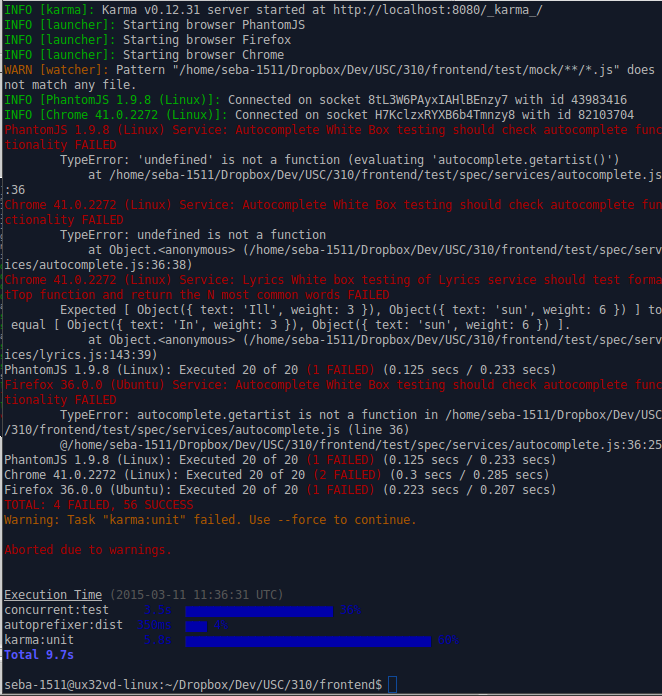
\includegraphics{karma.png}
\caption{Karma Unit Tests Results}
\end{figure}

\subsection{2.2 PHPUnit Testing
Software}\label{phpunit-testing-software}

The PHPUnit software was used to run unit testing on the backend PHP
code. These tests were mainly geared towards achieving milestones for
the autocomplete functionality and gathering the word cloud data
(milestones G.1 and G.2 of the PMP). The following list describes each
test that was run with the PHPUnit software:

\begin{itemize}
\itemsep1pt\parskip0pt\parsep0pt
\item
  Test 1: testQueryArtist()

  \begin{itemize}
  \itemsep1pt\parskip0pt\parsep0pt
  \item
    Milestone G.1
  \item
    Ensures that, given a correct artist name, the autocomplete returns
    results that are not empty
  \end{itemize}
\item
  Test 2: testQueryArtistSize()

  \begin{itemize}
  \itemsep1pt\parskip0pt\parsep0pt
  \item
    Milestone G.1
  \item
    Given a correct artist name, ensures that autocomplete returns the
    correct number of results
  \end{itemize}
\item
  Test 3: testQueryArtistError()

  \begin{itemize}
  \itemsep1pt\parskip0pt\parsep0pt
  \item
    Milestone G.1
  \item
    Given an invalid input, ensures that autocomplete returns null
    instead of incorrect data
  \end{itemize}
\item
  Test 4: testGetApiKey()

  \begin{itemize}
  \itemsep1pt\parskip0pt\parsep0pt
  \item
    Milestone G.1
  \item
    Testing to make sure the EchoNest API key is correct and not empty
  \end{itemize}
\item
  Test 5: testGetClient()

  \begin{itemize}
  \itemsep1pt\parskip0pt\parsep0pt
  \item
    Milestone G.1
  \item
    Ensures that a client connection to the databases can be established
    using the API key
  \end{itemize}
\item
  Test 6: testGetArtistApi()

  \begin{itemize}
  \itemsep1pt\parskip0pt\parsep0pt
  \item
    Milestone G.1
  \item
    Checks that a client connection to the artist API is valid
  \end{itemize}
\item
  Test 7: testGetArtist()

  \begin{itemize}
  \itemsep1pt\parskip0pt\parsep0pt
  \item
    Milestone G.2
  \item
    Ensures that, given an artist name, the webscraper receives the
    right artist name
  \end{itemize}
\item
  Test 8: testGetUrlList()

  \begin{itemize}
  \itemsep1pt\parskip0pt\parsep0pt
  \item
    Milestone G.2
  \item
    Confirms that gathering URL's of songs for a given valid artist name
    functions properly
  \end{itemize}
\item
  Test 9: testGetUrlListSize()

  \begin{itemize}
  \itemsep1pt\parskip0pt\parsep0pt
  \item
    Milestone G.2
  \item
    Given a valid artist name, ensures that the webscraper returns the
    correct number of URL links for songs
  \end{itemize}
\item
  Test 10: testGetUrlListEmpty()

  \begin{itemize}
  \itemsep1pt\parskip0pt\parsep0pt
  \item
    Milestone G.2
  \item
    Given an empty artist name, ensures that the webscraper returns zero
    URL links
  \end{itemize}
\item
  Test 11: testGetUrlListFaultyInput()

  \begin{itemize}
  \itemsep1pt\parskip0pt\parsep0pt
  \item
    Milestone G.2
  \item
    Given faulty artist name input, ensures that the webscraper returns
    zero URL links (no bad outputs)
  \end{itemize}
\item
  Test 12: testGetLyrics()

  \begin{itemize}
  \itemsep1pt\parskip0pt\parsep0pt
  \item
    Milestone G.2
  \item
    Given a valid artist name, asserts that the lyrics list will not be
    empty and equals the correct number of songs
  \end{itemize}
\item
  Test 13: testGetLyricsFaultyInput()

  \begin{itemize}
  \itemsep1pt\parskip0pt\parsep0pt
  \item
    Milestone G.2
  \item
    Given faulty artist name input, ensures that the lyrics list
    contains no results and throws an error code
  \end{itemize}
\item
  Test 14: testGetLyricsEmpty()

  \begin{itemize}
  \itemsep1pt\parskip0pt\parsep0pt
  \item
    Milestone G.2
  \item
    Given no artist name input, ensures that the lyrics list contains no
    results and returns an error message
  \end{itemize}
\item
  Test 15: testScrapeBetween()

  \begin{itemize}
  \itemsep1pt\parskip0pt\parsep0pt
  \item
    Milestone G.2
  \item
    Given a HTML page, ensures that the webscraper functions properly
    and takes the correct data from the site
  \end{itemize}
\end{itemize}

\begin{figure}[htbp]
\centering
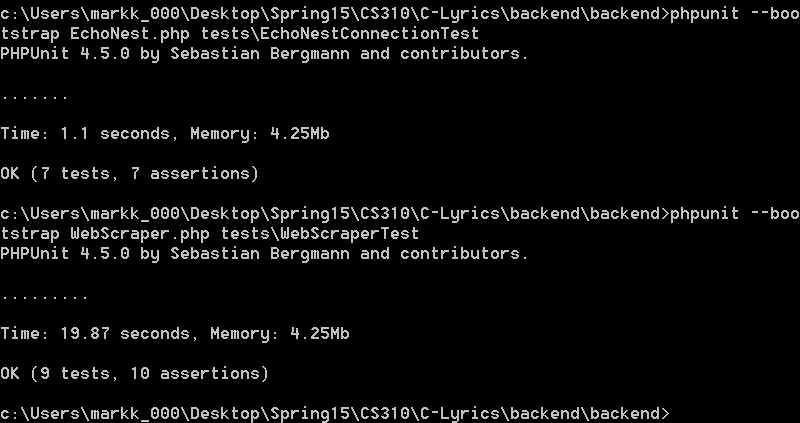
\includegraphics{phpunit.png}
\caption{PHPUnit Tests Results}
\end{figure}

\subsection{2.3 Measures and
Coverage}\label{measures-and-coverage}

\begin{figure}[htbp]
\centering
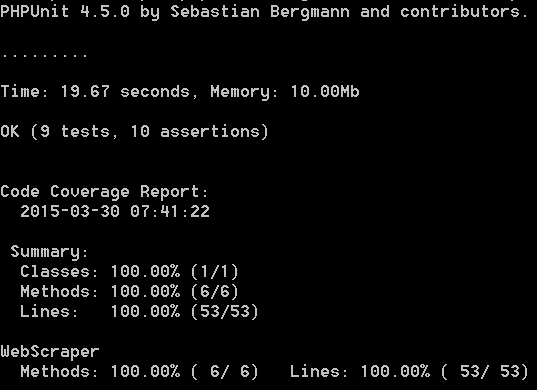
\includegraphics{coverage1.png}
\caption{Code Coverage, part 1}
\end{figure}

The tests run using Karma software sufficiently cover all of the
functionalities for the JavaScript frontend. Only certain functions were
tested since the majority of the code calls functions without specific
testable return output. The testing code written actively covers these
functions by ensuring that larger, encompassing functionalities are
working properly.

\begin{figure}[htbp]
\centering
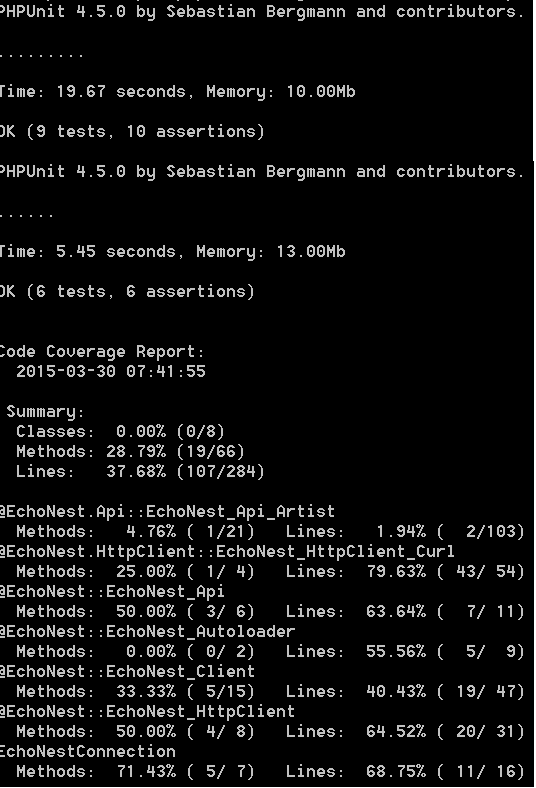
\includegraphics{codeCoverage2.png}
\caption{Code Coverage, part 2}
\end{figure}

The PHPUnit tests that were run have sufficiently explored each
necessary function of the PHP backend. By checking how the code
processes various types of inputs (valid, faulty, and empty) as well as
checking the communication of different components of the code, we can
be sure that the code will not provide functional errors in the
processes of generating autocomplete results as well as pulling song
lists and lyrics from lyric websites. In this test, we have run 15 tests
to measure the robustness of the code. All of them have executed without
errors, providing sufficient evidence that the PHP code runs properly.

XDebug along with PHPUnit were used to measure code coverage for the
back end. The first set of tests, which tests the web scraper
functionality, returns 100\% coverage in regards to the class itself,
lines of code, and methods. The second set of tests, which tests the
EchoNest API connection and transfer of autocomplete results, returns
71.43\% coverage. The coverage test itself produces other coverage
results, but those results result from using a 3rd party class that
connects to the API. It is assumed that the 3rd party class has properly
tested the class before public release, so while parts of the API code
code are not covered in these tests, it's functionality should already
be at 100\%.

\section{3 Acceptance Testing}\label{acceptance-testing}

\begin{figure}[htbp]
\centering
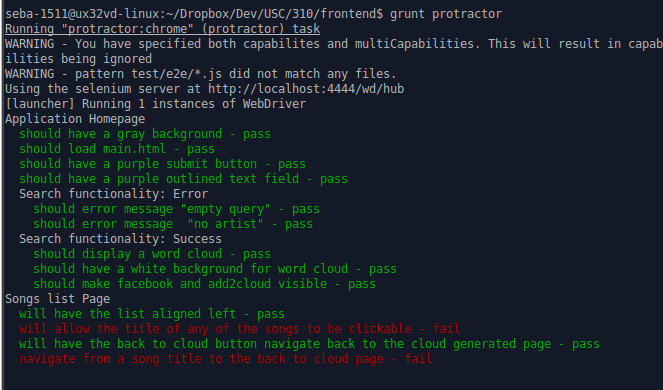
\includegraphics{protractor.png}
\caption{Protractor Acceptance Tests Results}
\end{figure}

\subsection{3.1 Protractor Testing
Environment}\label{protractor-testing-environment}

Protractor is a testing framework used to run end-to-end type tests for
AngularJS implementations. These tests will be used as acceptance tests
since they reveal if the user defined requirements as described in the
SRS are met. The nature of Protractor code makes it difficult to state
tests by function name as was done in the previous section. To
compensate, the criteria for each unit tests are listed below, the path
to each test on the Github repository is also given for further
reference.

The procedure to implement acceptance tests was to have a test for each
requirement defined in the SRS. Once that mapping was done, tests were
created so as to simulate actions a user would perform and ensure that
the application always provided a decent rendering. This was
accomplished by clicking on buttons, submitting text to input fields.
After each one of these actions tests expect a predefined element to
exist, to have a certain color or a given shape. Some of those tests
currently do not pass for unimplemented functionalities.

\begin{itemize}
\itemsep1pt\parskip0pt\parsep0pt
\item
  Main Page Layout (frontend/test/spec/controller/main.js)

  \begin{itemize}
  \itemsep1pt\parskip0pt\parsep0pt
  \item
    Milestone G
  \item
    Test that the first page when opened has search bar
  \item
    Grey background
  \item
    Submit button purple
  \item
    Text field outlined in purple
  \end{itemize}
\item
  Search (frontend/test/spec/controller/main.js)

  \begin{itemize}
  \itemsep1pt\parskip0pt\parsep0pt
  \item
    Milestone G.2
  \item
    If input artist name that doesn't exist

    \begin{itemize}
    \itemsep1pt\parskip0pt\parsep0pt
    \item
      Error ``Artist not found''
    \item
      Empty submit error
    \item
      Facebook and Add to Cloud not on screen
    \end{itemize}
  \item
    If artist's name correct

    \begin{itemize}
    \itemsep1pt\parskip0pt\parsep0pt
    \item
      Word cloud appears
    \item
      White background appears
    \item
      ``Add to Cloud'' appears
    \item
      ``Facebook Share'' appears
    \end{itemize}
  \end{itemize}
\item
  Autocomplete (frontend/test/spec/controller/main.js)

  \begin{itemize}
  \itemsep1pt\parskip0pt\parsep0pt
  \item
    Milestone G.1
  \item
    After pause in user's input to search bar autocomplete field becomes
    visible
  \item
    Test scroll bar
  \item
    Pictures for each artist
  \end{itemize}
\item
  Word Cloud (frontend/test/spec/controller/main.js)

  \begin{itemize}
  \itemsep1pt\parskip0pt\parsep0pt
  \item
    Milestone G.2
  \item
    Word size depends on frequency
  \item
    Words multicolored
  \item
    Words link to songs list page
  \item
    Stop words filtered out (ex. ``it,'' ``the,'' and ``a'')
  \item
    Word cloud generation is 10 sec - 1 min
  \end{itemize}
\item
  Song List (frontend/test/spec/controller/songlist.js)

  \begin{itemize}
  \itemsep1pt\parskip0pt\parsep0pt
  \item
    Milestone H
  \item
    Songs sorted from highest frequency to lowest
  \item
    Ability to select a song title to go to lyrics page
  \item
    List will be aligned left
  \item
    Title is clickable
  \item
    Navigation buttons work

    \begin{itemize}
    \itemsep1pt\parskip0pt\parsep0pt
    \item
      ``Back to Cloud''
    \end{itemize}
  \end{itemize}
\item
  Lyrics (frontend/test/spec/controller/songlyrics.js)

  \begin{itemize}
  \itemsep1pt\parskip0pt\parsep0pt
  \item
    Milestone I
  \item
    Selected word highlighted
  \item
    Lyrics will be aligned left
  \item
    Navigation buttons work

    \begin{itemize}
    \itemsep1pt\parskip0pt\parsep0pt
    \item
      ``Back to Cloud''
    \item
      ``Back to Songs''
    \end{itemize}
  \end{itemize}
\end{itemize}

\subsection{3.2 Measures and
Coverage}\label{measures-and-coverage-1}

There is one black-box test for every requirement. One test is enough
since there are a set number of pages and functions (buttons) that the
user has access to. The tests will figure out for example, if the add to
cloud button works. Adding lyrics to the cloud is a requirement, the
test will check if the connection is made. The correctness of what
actually shows up in the cloud once new lyrics are added is a white-box
testing problem. White-box testing concerns are handled in the previous
section of this document. Therefore, our testing policy assumes that as
long as each customer requirement is tested at least once, we have
achieved satisfactory test coverage.

Furthermore, the development team does not have enough resources to test
each requirement more than once. The product will also not be delivered
on time if a more comprehensive testing regimen is applied for
acceptance testing procedures.

\section{4 Quality Testing}\label{quality-testing}

\subsection{4.1 Reliability Tests}\label{reliability-tests}

In the SRS we stated that we would test the reliability of our product
based on the percent accuracy over 1500 searches, the minimum required
percent being 95 percent and the goal being 98 percent. During testing
we decided that it was not feasible and unnecessary for us to run the
program 1500 times in order to gauge the reliability of our system given
time and resource constraints. Instead, we tested our system by
searching for distinct 15 artists across different genres running each
search 3 times to ensure that it is reliably accurate. Because we are
grabbing all of our artist and lyric information from the API, it can be
assumed that our system will also work for all remaining artists in the
API's database.

\subsection{4.2 Availability Tests}\label{availability-tests}

The SRS states that we will test the availability of our system by the
percentage of time that it is available out of 80 hours of monitoring
the system, 95 percent of the time being the minimum required and 97
percent of the time being the goal. This was simulated by having each of
the six members of the development team monitor the system for roughly
13 hours adding up to a total of 80 hours that the system was monitored.
The system was not only monitored using different OSs but also using
different web browsers such as Chrome, Firefox and PhantomJS. We feel
that this is sufficient proof that our system will be available as
needed and that this test also fulfills all application testability
requirements.

\subsection{4.3 Other Quality Tests}\label{other-quality-tests}

Other forms of quality testing such as maintenance tests and security
tests were not administered because they did not fits the needs of this
project. Because there is no projected maintenance for this project and
there are no foreseeable security risks, we feel that it is appropriate
to omit them.

\section{5 Testing Compliances with
PMP}\label{testing-compliances-with-pmp}

\subsection{5.1 Quality Assurance
Testing}\label{quality-assurance-testing}

For quality assurance purposes, deviations from the PMP were noted in
section 3.3.3 and 3.3.4 of the Implementation document. Due to changes
in delivery schedule, we did not have the necessary time to achieve full
coverage of the test cases.

\subsection{5.2 Risk Monitoring}\label{risk-monitoring}

Risk monitoring was conducted regularly at all phases of testing. To
ensure that the maximum number of EchoNest queries was not met during
testing, we made sure to write test cases that were robust and covered
multiple features whenever possible. This was the main consideration
that was marked out in the PMP. All general risk monitoring practices
that were outlined (such as risks not related specifically to
implementation) were continually met throughout the testing phase of the
project.

\section{6 Appendices}\label{appendices}

\subsection{6.1 Declaration of
Milestones}\label{declaration-of-milestones}

The milestones below were conceived for and reported on the PMP
document. The below table is an excerpt from the original PMP document.
They are reproduced here for clarity and reference.

\begin{itemize}
\itemsep1pt\parskip0pt\parsep0pt
\item
  Testing and Final
  Delivery\ldots{}..\ldots{}\ldots{}\ldots{}\ldots{}\ldots{}\ldots{}\ldots{}\ldots{}\ldots{}\ldots{}..\ldots{}\ldots{}\ldots{}\ldots{}3/11/15*
\item
  Milestones G-J

  \begin{itemize}
  \itemsep1pt\parskip0pt\parsep0pt
  \item
    G: Testing of the Home Page

    \begin{itemize}
    \itemsep1pt\parskip0pt\parsep0pt
    \item
      G.1: Search bar with autocomplete functionality when typing in an
      artist's name
    \item
      G.2: WC generation with words that can be selected to take the
      user to the Songs Page
    \item
      G.3: Share button to upload the WC to Facebook
    \item
      G.4: Add to Cloud button to create a new WC based off of words
      commonly used by both of the specified artists
    \end{itemize}
  \item
    H: Testing of the Songs Page

    \begin{itemize}
    \itemsep1pt\parskip0pt\parsep0pt
    \item
      H.1: List of songs sorted by how frequently the selected word is
      used in each song
    \item
      H.2: Song titles in list able to be selected, taking the user to
      the Lyrics page
    \item
      H.3: Back to Home button takes the user back to the Home Page with
      the WC still displayed and the artist's name still in the Search
      Bar
    \end{itemize}
  \item
    I: Testing of the Lyrics Page

    \begin{itemize}
    \itemsep1pt\parskip0pt\parsep0pt
    \item
      I.1: Lyrics displayed on page with the selected word highlighted
      every time it appears in the song
    \item
      I.2: Back to Songs button takes the user back to the Songs Page
      with the same list of songs still displayed in the same order
    \item
      I.3: Back to Home button takes the user back to the Home Page with
      the WC still displayed and the artist's name still in the Search
      Bar
    \end{itemize}
  \item
    J: Testing of the entire product to ensure all pages work together
    as specified in the SRS
  \end{itemize}
\end{itemize}

\subsection{6.2 Deviations From PMP}\label{deviations-from-pmp}

\subsubsection{6.2.1 Deviations from
Schedule}\label{deviations-from-schedule}


\begin{figure}[htbp]
\centering
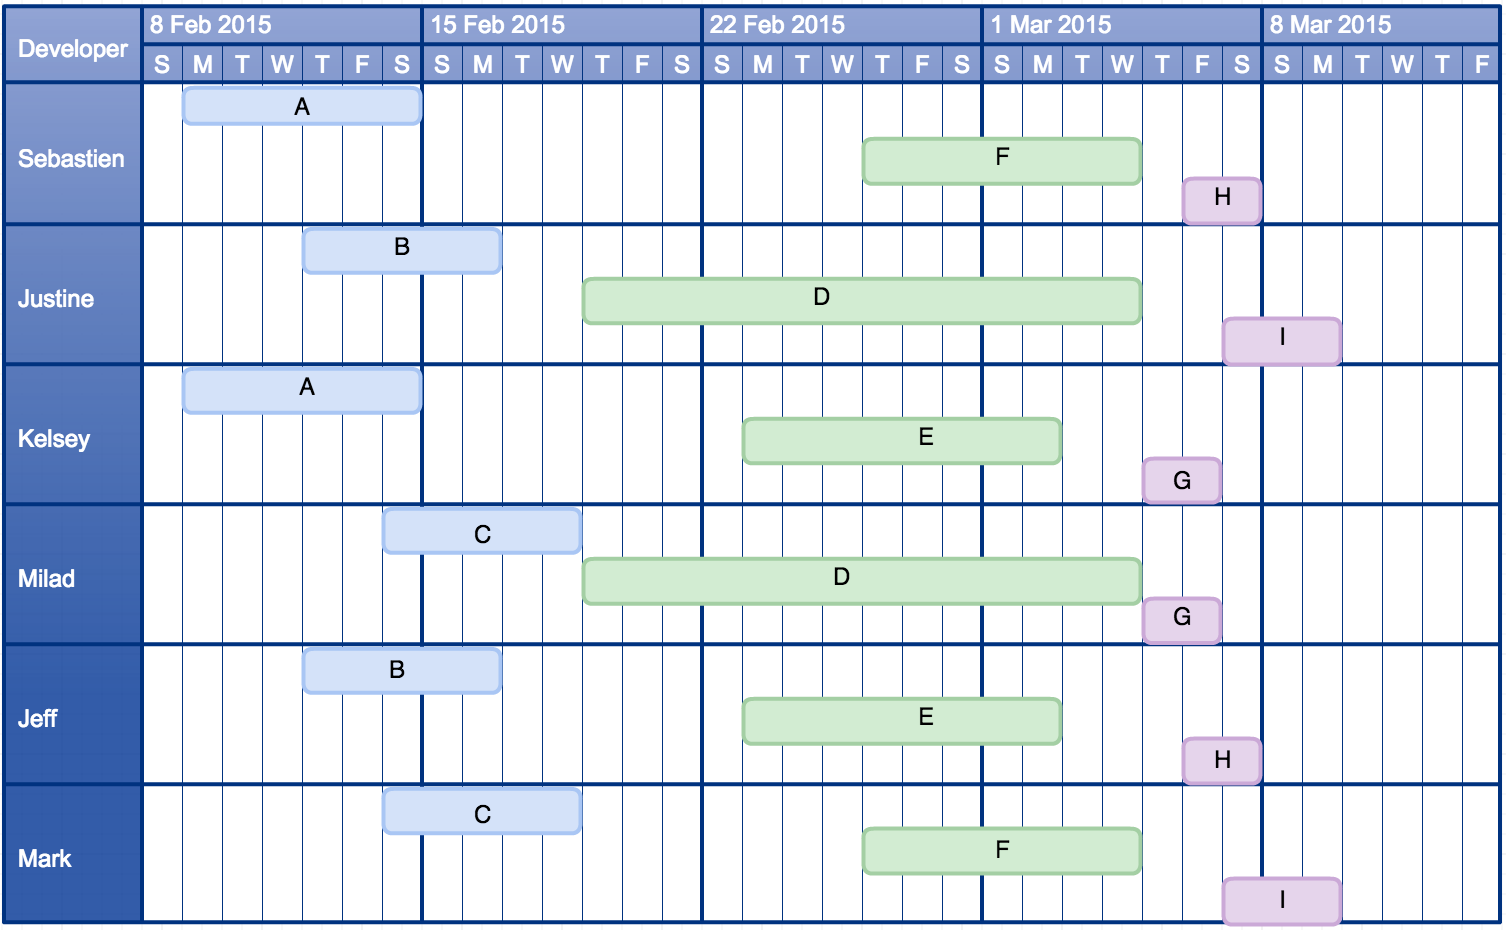
\includegraphics{StaffAllocation.png}
\caption{Staff Allocation}
\end{figure}

Originally, milestones were organized according to the table below,
where each letter corresponds to a mile stone in each phase of the
Waterfall software development cycle. The Milestones of interest are
letter G-J. A description of milestones G-J can be found in the previous
appendix 5.1. Significant deviation has occurred in project schedule
cause by changed deliverable due dates.

The client pushed up the deadline for the testing document delivery to
Wednesday March 11 2015. Therefore, milestones G-J should be extended
until that date in the image above, representing the change in our PMP.

\subsubsection{6.2.2 Deviations From Milestone
Planning}\label{deviations-from-milestone-planning}

Team member Milad Gueramian was unable to contribute to testing
activities due to loss of development equipment (laptop computer).
Therefore, he was unassigned from milestone G and was given the task of
completing and preparing the testing document. A milestone was created
for this task in the Github Issue tracker tool which, as described in
the PMP, is use to coordinate and keep track of development team
activities.

Furthermore, team member Jeff Kang was also reassigned to create the
testing document with Milad Gueramian as the difficulty and resource
usage of this task was not considered in the PMP.

\subsection{6.3 Screenshots}\label{screenshots}

Here are the screenshots of the application as tested in a mobile browser and a desktop one.

\begin{figure}[htbp]
\centering
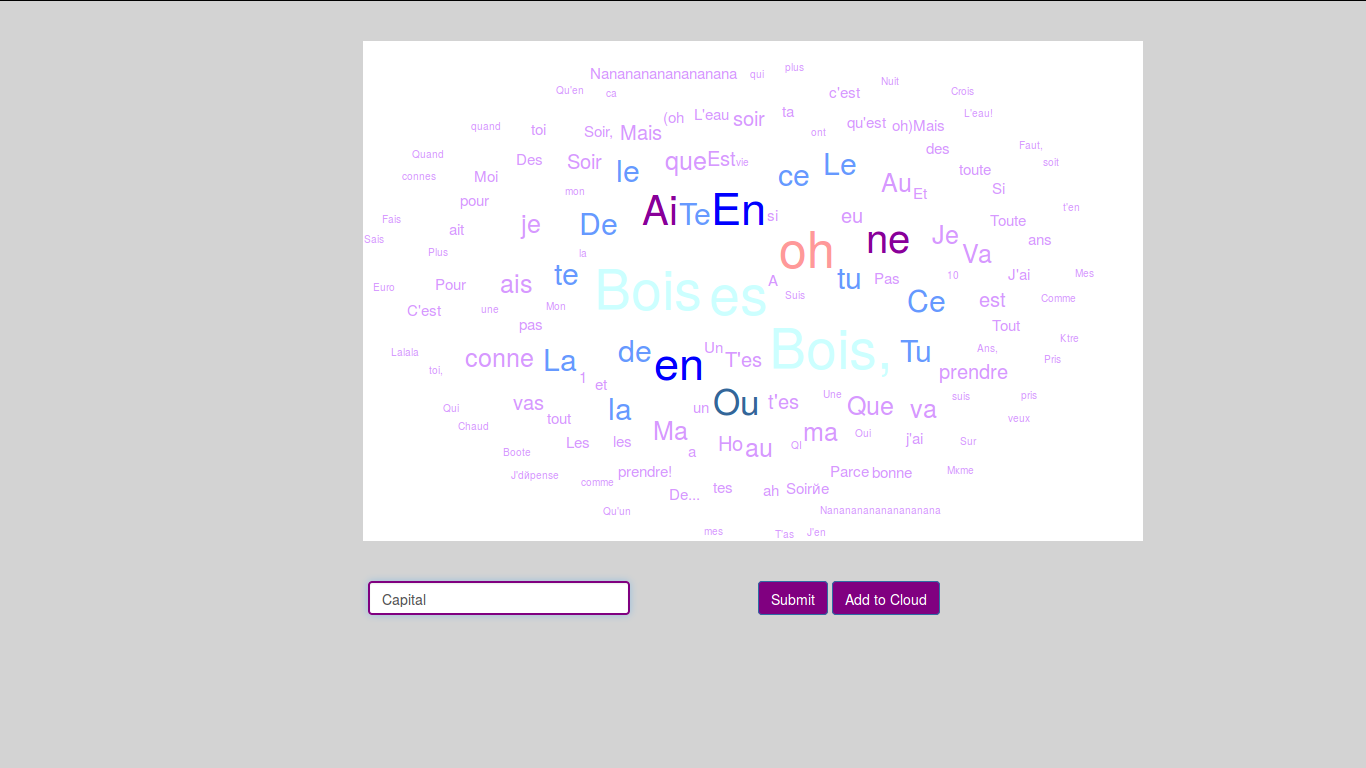
\includegraphics{desktop.png}
\caption{Desktop View}
\end{figure}

\begin{figure}[htbp]
\centering
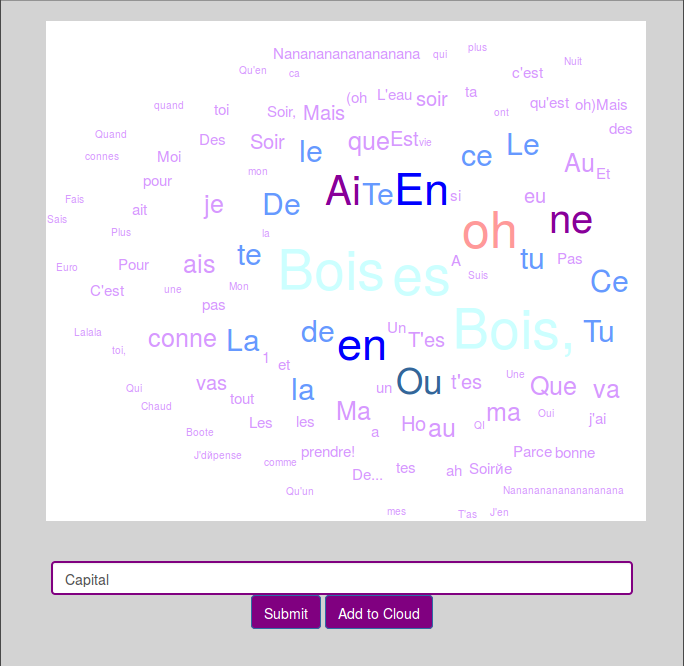
\includegraphics{mobile.png}
\caption{Mobile View}
\end{figure}


\end{document}
